
\begin{figure}[h!]
\centering
\caption{Ingresos del GNC}
\label{fig:Ingreso}
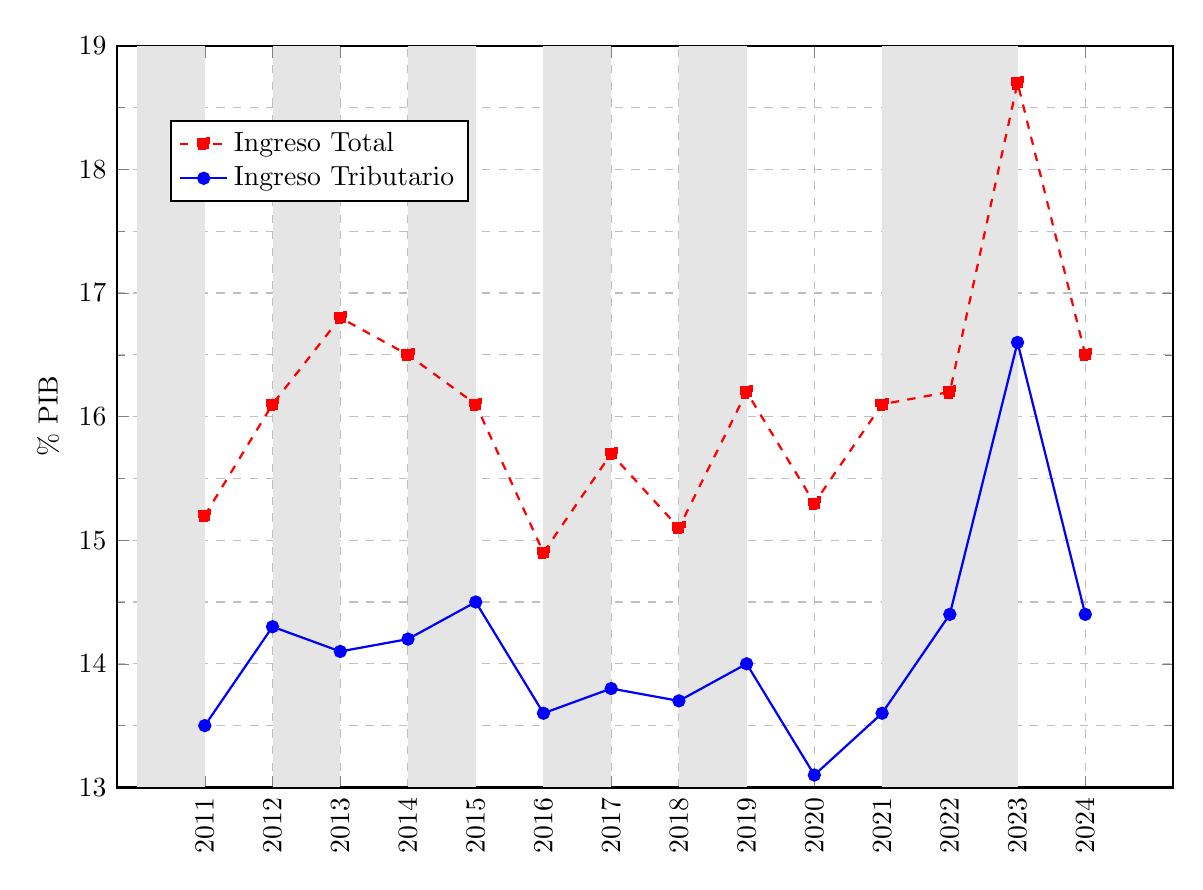
\begin{tikzpicture}
\begin{axis}[
    width=15cm,
    height=11cm,
%    xlabel={Años},
    ylabel={\% PIB},
    xtick=data,
    xticklabels={
        {2011}, {2012}, {2013}, {2014}, {2015}, {2016}, {2017}, {2018}, {2019}, {2020}, {2021},
        {2022}, {2023}, {2024} 
    },
    x tick label style={rotate=90, anchor=east},
    ymin=13,
    ymax=19,
    grid=major,
    grid=both,
    grid style=dashed,
    minor y tick num=1,
    legend style={at={(0.05,0.9)}, anchor=north west},
    legend cell align={left},
    thick
]


% Sombra en 2011 (Ley 1430 de 2010)
\draw [fill=gray!20, draw=none] (axis cs:06,13) rectangle (axis cs:07,19);
% Sombra en 2013 (Ley 1607 de 2012)
\draw [fill=gray!20, draw=none] (axis cs:08,13) rectangle (axis cs:09,19);
% Sombra en 2015 (Ley 1739 de 2014)
\draw [fill=gray!20, draw=none] (axis cs:10,13) rectangle (axis cs:11,19);
% Sombra en 2017 (Ley 1819 de 2016)
\draw [fill=gray!20, draw=none] (axis cs:12,13) rectangle (axis cs:13,19);

% Sombra en 2019 (Ley 1943 de 2018 (Inexequible))
\draw [fill=gray!20, draw=none] (axis cs:14,13) rectangle (axis cs:15,19);
%% Sombra en 2020 (Ley 2010 de 2019)
%\draw [fill=gray!20, draw=none] (axis cs:15,13) rectangle (axis cs:16,19);
% Sombra en 2022 (Ley 2155 de 2021)
\draw [fill=gray!20, draw=none] (axis cs:17,13) rectangle (axis cs:18,19);
% Sombra en 2023 (Ley 2277 de 2022)
\draw [fill=gray!20, draw=none] (axis cs:18,13) rectangle (axis cs:19,19);


% Datos de Ingresos Totales de la Nación
\addplot[
    mark=square*,
    dashed,
    red
] coordinates {
    (7,15.2) (8,16.1) 
    (9,16.8) (10,16.5) (11,16.1) (12,14.9) (13,15.7) (14,15.1) (15,16.2) (16,15.3) 
    (17,16.1) (18,16.2) (19,18.7) (20,16.5)
};

%Datos de Ingresos Tributarios
\addplot[
    mark=*,
    solid,
    blue
] coordinates {
    (7,13.5) (8,14.3) 
    (9,14.1) (10,14.2) (11,14.5) (12,13.6) (13,13.8) (14,13.7) (15,14.0) (16,13.1) 
    (17,13.6) (18,14.4) (19,16.6) (20,14.4)
};

\legend{Ingreso Total, Ingreso Tributario}
\end{axis}
\end{tikzpicture}
\\ \footnotesize{\textit{Fuente: Elaboración propia con base en \textcite{minhacienda_balance_2025}.}}
\end{figure}
